\documentclass[aspectratio=169,10pt]{beamer}

\usetheme[numbering=fraction,progressbar=frametitle,block=fill]{metropolis}
\geometry{papersize={192mm,108mm}}
\usefonttheme[onlymath]{serif}
\usepackage{amsmath,amssymb,bm,booktabs,array}
\usepackage{tikz,pgfplots,listings}
\pgfplotsset{compat=1.17}
\usetikzlibrary{arrows.meta,positioning,calc,fit,backgrounds,decorations.pathreplacing,matrix}

% ---------------------------------------------------------------- colours
% One colour per stage, used consistently in every diagram.
\definecolor{cInk}{HTML}{22303C}
\definecolor{cTok}{HTML}{5B6770}   % tokens / ids
\definecolor{cEmb}{HTML}{2F6DB5}   % embeddings
\definecolor{cAtt}{HTML}{D9822B}   % attention
\definecolor{cFfn}{HTML}{2E8B57}   % feed-forward
\definecolor{cNrm}{HTML}{8C7A2B}   % normalisation
\definecolor{cOut}{HTML}{7B4FA6}   % output / sampling
\definecolor{cBad}{HTML}{B03A3A}
\setbeamercolor{normal text}{fg=cInk,bg=white}
\setbeamercolor{frametitle}{bg=cInk,fg=white}
\setbeamercolor{progress bar}{fg=cAtt,bg=cAtt!25}
\setbeamercolor{alerted text}{fg=cAtt}
\setbeamercolor{block title}{bg=cEmb!14,fg=cInk}
\setbeamercolor{block body}{bg=cEmb!5}
\setbeamerfont{block title}{series=\bfseries,size=\small}
\setbeamertemplate{itemize item}{\color{cAtt}\rule[0.25ex]{0.9ex}{0.9ex}}
\setbeamertemplate{itemize subitem}{\color{cTok}--}
\setlength{\leftmargini}{1.1em}

% ---------------------------------------------------------------- macros
\newcommand{\R}{\mathbb{R}}
\DeclareMathOperator{\softmax}{softmax}
\newcommand{\T}{\top}
\renewcommand{\cite}[1]{{\scriptsize\color{cTok}[#1]}}
\newcommand{\key}[1]{\textbf{\color{cAtt}#1}}

\tikzset{
  >={Stealth[length=5pt]},
  stage/.style={draw=#1,fill=#1!12,rounded corners=2pt,line width=0.7pt,
                minimum height=7.5mm,inner xsep=5pt,font=\small,align=center},
  stage/.default=cTok,
  flow/.style={->,line width=0.7pt,draw=cInk!80},
  note/.style={font=\scriptsize,text=cTok,align=center},
  tokbox/.style={draw=cTok,fill=cTok!10,rounded corners=1.5pt,font=\ttfamily\small,
                 minimum height=5.5mm,inner xsep=3pt,outer sep=0pt},
  cell/.style={minimum size=5mm,inner sep=0pt,font=\scriptsize},
}

\lstdefinestyle{py}{
  language=Python,basicstyle=\ttfamily\fontsize{6.1}{7.4}\selectfont,
  keywordstyle=\color{cEmb}\bfseries,commentstyle=\color{cFfn!85!black}\itshape,
  stringstyle=\color{cAtt!85!black},showstringspaces=false,columns=fullflexible,
  keepspaces=true,frame=none,backgroundcolor=\color{cInk!4},
  xleftmargin=3pt,xrightmargin=3pt,aboveskip=2pt,belowskip=2pt,
  literate={-}{{-}}1,
}


\DeclareMathOperator{\ReLU}{ReLU}
\newcommand{\num}[1]{\textbf{\color{cEmb}#1}}

% Graph Neural Networks from the Ground Up -- a 20-frame tutorial.
% Build from this directory:   latexmk -pdf gnn_tutorial.tex
% Figures read data written by ../experiments.py into generated/;
% frames 17 and 18 pull their listings directly from ../gcn_numpy.py, ../gnn.py and ../train.py.
\DeclareMathOperator{\AGG}{AGG}
\DeclareMathOperator{\UPD}{UPDATE}
\DeclareMathOperator{\MLP}{MLP}
\DeclareMathOperator{\LeakyReLU}{LeakyReLU}
\DeclareMathOperator{\diag}{diag}
\DeclareMathOperator{\mean}{mean}
\newcommand{\N}{\mathcal N}
\newcommand{\Ah}{\hat A}
\newcommand{\At}{\tilde A}
\newcommand{\Dt}{\tilde D}
\newcommand{\dt}{\tilde d}

% the 6-node example graph used on most slides: two triangles joined by the edge 3-4
\tikzset{
  gnode/.style={circle,draw=#1,fill=#1!15,line width=0.7pt,minimum size=6mm,inner sep=0pt,font=\footnotesize},
  gnode/.default=cEmb,
  gedge/.style={draw=cTok,line width=0.8pt},
  msg/.style={->,line width=1pt,draw=cAtt},
  dot/.style={circle,draw=#1,fill=#1!30,line width=0.5pt,minimum size=2.6mm,inner sep=0pt},
  dot/.default=cEmb,
}
\newcommand{\toycoords}{\coordinate (c1) at (0,0.85); \coordinate (c2) at (0,-0.85); \coordinate (c3) at (1.3,0);
  \coordinate (c4) at (2.8,0); \coordinate (c5) at (4.1,0.85); \coordinate (c6) at (4.1,-0.85);}
\newcommand{\toyedges}{\foreach \a/\b in {1/2,1/3,2/3,3/4,4/5,4/6,5/6} \draw[gedge] (n\a)--(n\b);}
\newcommand{\toygraph}{\toycoords \foreach \i in {1,...,6} \node[gnode] (n\i) at (c\i) {\i}; \toyedges}
% adjacency matrix as a grid of filled cells: #1 = list of r/c pairs (upper triangle), #2 = colour
\newcommand{\adjgrid}[2]{%
  \foreach \r/\c in {#1} {\fill[#2] (\c-1,-\r+1) rectangle ++(1,-1); \fill[#2] (\r-1,-\c+1) rectangle ++(1,-1);}
  \draw[cInk!35,line width=0.3pt] (0,0) grid (6,-6);
  \foreach \i in {1,...,6} {\node[font=\tiny,text=cTok] at (\i-0.5,0.5) {\i}; \node[font=\tiny,text=cTok] at (-0.5,-\i+0.5) {\i};}}

\title{Graph Neural Networks from the Ground Up}
\subtitle{Graphs as data, message passing, the GCN layer, depth and its limits, with runnable code}
\date{A 20-slide tutorial \textbullet{} companion code: \texttt{data.py}, \texttt{gcn\_numpy.py},
      \texttt{gnn.py}, \texttt{train.py}, \texttt{experiments.py}}

\newcommand{\coraNodes}{2{,}708}
\newcommand{\coraEdges}{5{,}278}
\newcommand{\coraFeatures}{1{,}433}
\newcommand{\coraClasses}{7}
\newcommand{\coraMeanDeg}{3.9}
\newcommand{\coraMedianDeg}{3}
\newcommand{\coraMaxDeg}{168}
\newcommand{\coraHomophily}{81}
\newcommand{\coraNonzero}{1.3}
\newcommand{\coraWordsPerPaper}{18}
\newcommand{\coraLabelledPct}{5.2}
\newcommand{\hopOneMean}{5}
\newcommand{\hopOnePct}{0.2}
\newcommand{\hopTwoMean}{37}
\newcommand{\hopTwoPct}{1.4}
\newcommand{\hopThreeMean}{128}
\newcommand{\hopThreePct}{5}
\newcommand{\hopFourMean}{373}
\newcommand{\hopFourPct}{14}
\newcommand{\hopEightMean}{1993}
\newcommand{\hopEightPct}{74}
\newcommand{\smoothZero}{0.06}
\newcommand{\smoothTwo}{0.22}
\newcommand{\smoothEight}{0.45}
\newcommand{\smoothSixtyFour}{0.80}
\newcommand{\coraGcnParams}{23{,}063}
\newcommand{\coraGcnSeedAcc}{80.7}
\newcommand{\coraGcnEpochs}{200}
\newcommand{\timeGcn}{5.0}
\newcommand{\coraMlpParams}{23{,}063}
\newcommand{\coraMlpSeedAcc}{58.9}
\newcommand{\coraMlpEpochs}{200}
\newcommand{\timeMlp}{3.8}
\newcommand{\coraGcnNoFeatParams}{43{,}463}
\newcommand{\coraGcnNoFeatSeedAcc}{72.0}
\newcommand{\coraGcnNoFeatEpochs}{200}
\newcommand{\timeGcnNoFeat}{2.8}
\newcommand{\coraSageParams}{46{,}103}
\newcommand{\coraSageSeedAcc}{78.9}
\newcommand{\coraSageEpochs}{193}
\newcommand{\timeSage}{4.6}
\newcommand{\coraGatParams}{92{,}373}
\newcommand{\coraGatSeedAcc}{81.5}
\newcommand{\coraGatEpochs}{200}
\newcommand{\timeGat}{9.9}
\newcommand{\coraGcnNoRegParams}{23{,}063}
\newcommand{\coraGcnNoRegSeedAcc}{79.7}
\newcommand{\coraGcnNoRegEpochs}{196}
\newcommand{\timeGcnNoReg}{2.6}
\newcommand{\coraLpMean}{69.6}
\newcommand{\coraLpStd}{3.4}
\newcommand{\coraMajorityMean}{10.5}
\newcommand{\coraMajorityStd}{0.8}
\newcommand{\coraGcnMean}{79.9}
\newcommand{\coraGcnStd}{1.3}
\newcommand{\coraMlpMean}{57.6}
\newcommand{\coraMlpStd}{2.4}
\newcommand{\coraGcnNoFeatMean}{66.1}
\newcommand{\coraGcnNoFeatStd}{3.3}
\newcommand{\coraSageMean}{78.3}
\newcommand{\coraSageStd}{2.1}
\newcommand{\coraGatMean}{79.7}
\newcommand{\coraGatStd}{2.0}
\newcommand{\coraGcnNoRegMean}{76.6}
\newcommand{\coraGcnNoRegStd}{1.6}
\newcommand{\coraSeeds}{10}
\newcommand{\coraGatSeeds}{5}
\newcommand{\gcnBeatsMlp}{10}
\newcommand{\gcnBeatsLp}{10}
\newcommand{\gcnBeatsSage}{7}
\newcommand{\gatBeatsGcn}{2}
\newcommand{\coraGcnFirstFiveMean}{79.7}
\newcommand{\coraGcnMin}{77.6}
\newcommand{\coraGcnMax}{81.3}
\newcommand{\gcnMinusMlp}{22}
\newcommand{\gcnBestEpoch}{196}
\newcommand{\gcnBestVal}{0.78}
\newcommand{\gcnFinalTrain}{0.41}
\newcommand{\noregFinalTrain}{0.018}
\newcommand{\noregBestVal}{0.67}
\newcommand{\mlpBestVal}{1.43}
\newcommand{\depthOne}{74.3}
\newcommand{\depthTrainOne}{97}
\newcommand{\depthResOne}{74.3}
\newcommand{\depthTwo}{79.7}
\newcommand{\depthTrainTwo}{99}
\newcommand{\depthResTwo}{79.7}
\newcommand{\depthThree}{77.8}
\newcommand{\depthTrainThree}{100}
\newcommand{\depthResThree}{77.8}
\newcommand{\depthFour}{72.8}
\newcommand{\depthTrainFour}{95}
\newcommand{\depthResFour}{77.3}
\newcommand{\depthFive}{42.8}
\newcommand{\depthTrainFive}{54}
\newcommand{\depthResFive}{74.5}
\newcommand{\depthSix}{41.6}
\newcommand{\depthTrainSix}{50}
\newcommand{\depthResSix}{72.8}
\newcommand{\depthSeven}{28.9}
\newcommand{\depthTrainSeven}{31}
\newcommand{\depthResSeven}{71.1}
\newcommand{\depthEight}{24.5}
\newcommand{\depthTrainEight}{24}
\newcommand{\depthResEight}{69.5}
\newcommand{\depthSeeds}{5}
\newcommand{\depthBest}{2}
\newcommand{\karateSeedWrong}{2}
\newcommand{\karateSeedWrongNodes}{2, 8}
\newcommand{\karateSeedAcc}{91.7}
\newcommand{\karateParams}{594}
\newcommand{\karateEpochs}{200}
\newcommand{\karateGcnMean}{95.6}
\newcommand{\karateGcnStd}{3.2}
\newcommand{\karateLpMean}{97.3}
\newcommand{\karateLpStd}{2.0}
\newcommand{\karateMajorityMean}{48.3}
\newcommand{\karateMajorityStd}{6.5}
\newcommand{\karateMlpMean}{49.6}
\newcommand{\karateMlpStd}{11.4}
\newcommand{\karateSeeds}{20}
\newcommand{\karateGcnBeatsLp}{0}
\newcommand{\karateLpBeatsGcn}{8}
\newcommand{\experimentMinutes}{8}

\begin{document}

% ======================================================================= 1
\maketitle
\addtocounter{framenumber}{1}

% ======================================================================= 2
\begin{frame}{Why graphs? Data that is made of relations}
\begin{columns}[T,onlytextwidth]
\column{0.49\textwidth}
\small
Much data is not a table of independent rows. It is \textbf{things plus the relations between them}:
atoms joined by bonds, papers joined by citations, people joined by friendships.
A \key{graph} $G=(V,E)$ stores exactly that: a set of \textbf{nodes} $V$ and a set of
\textbf{edges} $E$ between pairs of nodes.

\vspace{1mm}
A \key{graph neural network} (GNN) is a network whose layers let every node combine its own
features with those of its neighbours. One small rule, applied at every node.
\column{0.48\textwidth}
\begin{block}{What the models we already know cannot do}
\footnotesize
\begin{itemize}
  \item \textbf{MLP}: wants a fixed-length vector per example and treats examples as independent.
        It has no input for ``who is connected to whom''.
  \item \textbf{CNN}: wants a regular grid, where every pixel has the same neighbours in the same
        places (up, down, left, right). A node in a graph has any number of neighbours, in no order.
\end{itemize}
\end{block}
\end{columns}
\vspace{1.5mm}
\centering
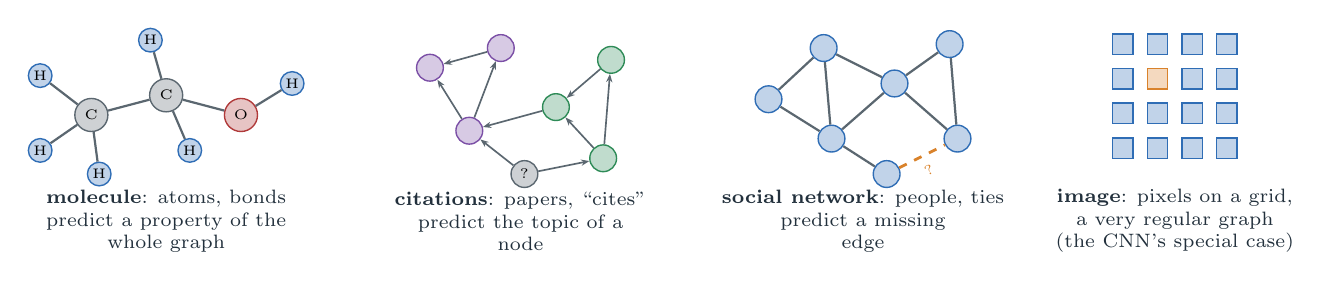
\begin{tikzpicture}[font=\scriptsize]
  % ---- molecule (ethanol heavy atoms + hydrogens)
  \begin{scope}[shift={(0,0)}]
    \node[dot=cTok,minimum size=4.2mm,font=\tiny] (C1) at (0,0) {C};
    \node[dot=cTok,minimum size=4.2mm,font=\tiny] (C2) at (0.95,0.25) {C};
    \node[dot=cBad,minimum size=4.2mm,font=\tiny] (O) at (1.9,0) {O};
    \foreach \n/\x/\y in {a/-0.65/0.5,b/-0.65/-0.45,c/0.1/-0.75,d/0.75/0.95,e/1.25/-0.45,f/2.55/0.4}
      \node[dot=cEmb,minimum size=3mm,font=\fontsize{4}{4}\selectfont] (H\n) at (\x,\y) {H};
    \foreach \a/\b in {C1/C2,C2/O,C1/Ha,C1/Hb,C1/Hc,C2/Hd,C2/He,O/Hf} \draw[gedge] (\a)--(\b);
    \node[note,text=cInk] at (0.95,-1.35) {\textbf{molecule}: atoms, bonds\\predict a property of the\\whole graph};
  \end{scope}
  % ---- citation network
  \begin{scope}[shift={(4.3,0)}]
    \foreach \n/\x/\y/\c in {a/0/0.6/cOut,b/0.9/0.85/cOut,c/0.5/-0.2/cOut,d/1.6/0.1/cFfn,e/2.3/0.7/cFfn,f/2.2/-0.55/cFfn,g/1.2/-0.75/cTok}
      \node[dot=\c,minimum size=3.4mm] (\n) at (\x,\y) {};
    \foreach \a/\b in {b/a,c/a,c/b,d/c,e/d,f/d,f/e,g/c,g/f} \draw[->,>={Stealth[length=3pt]},draw=cTok,line width=0.6pt] (\a)--(\b);
    \node[font=\tiny] at (g) {?};
    \node[note,text=cInk] at (1.15,-1.35) {\textbf{citations}: papers, ``cites''\\predict the topic of a\\node};
  \end{scope}
  % ---- social network
  \begin{scope}[shift={(8.6,0)}]
    \foreach \n/\x/\y in {a/0/0.2,b/0.7/0.85,c/0.8/-0.3,d/1.6/0.4,e/2.3/0.9,f/2.4/-0.3,g/1.5/-0.75}
      \node[dot=cEmb,minimum size=3.4mm] (\n) at (\x,\y) {};
    \foreach \a/\b in {a/b,a/c,b/c,b/d,c/d,d/e,d/f,e/f,c/g} \draw[gedge] (\a)--(\b);
    \draw[cAtt,dashed,line width=1pt] (g)-- node[below,sloped,font=\tiny,text=cAtt]{?} (f);
    \node[note,text=cInk] at (1.2,-1.35) {\textbf{social network}: people, ties\\predict a missing\\edge};
  \end{scope}
  % ---- image as a grid graph
  \begin{scope}[shift={(13.1,-0.42)},x=4.4mm,y=4.4mm]
    \foreach \i in {0,...,3} \foreach \j in {0,...,3} \node[dot=cEmb,minimum size=2.6mm,rectangle] (p\i\j) at (\i,\j) {};
    \foreach \i in {0,...,3} \foreach \j [evaluate=\j as \k using int(\j+1)] in {0,1,2} {\draw[gedge,line width=0.5pt] (p\i\j)--(p\i\k); \draw[gedge,line width=0.5pt] (p\j\i)--(p\k\i);}
    \node[dot=cAtt,minimum size=2.6mm,rectangle] at (1,2) {};
    \node[note,text=cInk] at (1.5,-2.1) {\textbf{image}: pixels on a grid,\\a very regular graph\\(the CNN's special case)};
  \end{scope}
\end{tikzpicture}

\vspace{1mm}
\raggedright\footnotesize
\textbf{Do the relations carry information?} In the Cora citation network used later
(\coraNodes{} papers, \coraEdges{} citation links, \coraClasses{} topics), \coraHomophily\% of the links join two
papers on the \emph{same} topic. A paper's neighbours say a lot about it. Slide 19 measures how much
a model gains by using them. Surveys: \cite{17}; origins: \cite{1}.
\end{frame}

% ======================================================================= 3
\begin{frame}{Representing a graph: edge list, $A$, $D$ and $X$}
\begin{columns}[T,onlytextwidth]
\column{0.47\textwidth}
\centering
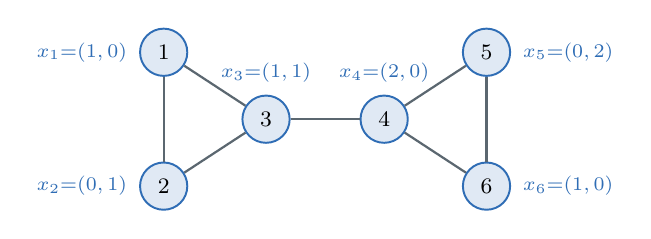
\begin{tikzpicture}
  \toygraph
  \node[note,text=cEmb,left=0.3mm of n1] {$x_1{=}(1,0)$}; \node[note,text=cEmb,left=0.3mm of n2] {$x_2{=}(0,1)$};
  \node[note,text=cEmb,above=0.3mm of n3] {$x_3{=}(1,1)$}; \node[note,text=cEmb,above=0.3mm of n4] {$x_4{=}(2,0)$};
  \node[note,text=cEmb,right=0.3mm of n5] {$x_5{=}(0,2)$}; \node[note,text=cEmb,right=0.3mm of n6] {$x_6{=}(1,0)$};
\end{tikzpicture}

\vspace{0.5mm}
{\scriptsize\color{cTok}The running example: 6 nodes, 7 edges, 2 features per node.}
\vspace{-1mm}
{\footnotesize
\[
 A=\begin{bmatrix}
 0&1&1&0&0&0\\ 1&0&1&0&0&0\\ 1&1&0&1&0&0\\ 0&0&1&0&1&1\\ 0&0&0&1&0&1\\ 0&0&0&1&1&0
 \end{bmatrix}\!,\;
 d=\begin{bmatrix}2\\2\\3\\3\\2\\2\end{bmatrix}\!,\;
 X=\begin{bmatrix}1&0\\0&1\\1&1\\2&0\\0&2\\1&0\end{bmatrix}
\]}
\vspace{-2mm}
{\footnotesize \textbf{Edge list}: $(1,2),(1,3),(2,3),(3,4),(4,5),(4,6),(5,6)$}
\column{0.50\textwidth}
\footnotesize
\begin{itemize}
  \item \key{Adjacency matrix} $A\in\{0,1\}^{n\times n}$: $A_{vu}=1$ if an edge joins $v$ and $u$.
        Row $v$ lists the \key{neighbours} $\N(v)$ of $v$.
  \item \key{Degree} $d_v=\sum_u A_{vu}=|\N(v)|$, \ $D=\diag(d)$. Check: $\sum_v d_v=14=2|E|$.
  \item \key{Node features} $X\in\R^{n\times F}$: row $v$ describes node $v$ (the words of a paper,
        the type of an atom). No features? Use $X=I$, a one-hot id per node.
  \item \textbf{Undirected}: $A=A^\T$ (friendship, bonds). \textbf{Directed}: $A_{vu}\ne A_{uv}$
        (``cites'', ``follows''). We symmetrise citations and work undirected.
  \item \key{Self-loop}: an edge from a node to itself, $A_{vv}=1$. Our data has none;
        slide 8 adds them on purpose.
\end{itemize}
\vspace{-1mm}
\begin{block}{Real graphs are sparse: store the edge list}
\footnotesize
Cora's $A$ has $2708^2\approx7.3$ million entries; only $2\times\coraEdges$ are non-zero (0.14\%).
Mean degree \coraMeanDeg, median \coraMedianDeg, maximum \coraMaxDeg. The code builds sparse matrices from
the edges (\texttt{graph\_operators}, \texttt{gnn.py}); a product $AH$ costs $O(|E|F)$, not $O(n^2F)$.
\end{block}
\end{columns}
\end{frame}

% ======================================================================= 4
\begin{frame}{Three kinds of prediction: node, edge, graph}
\centering
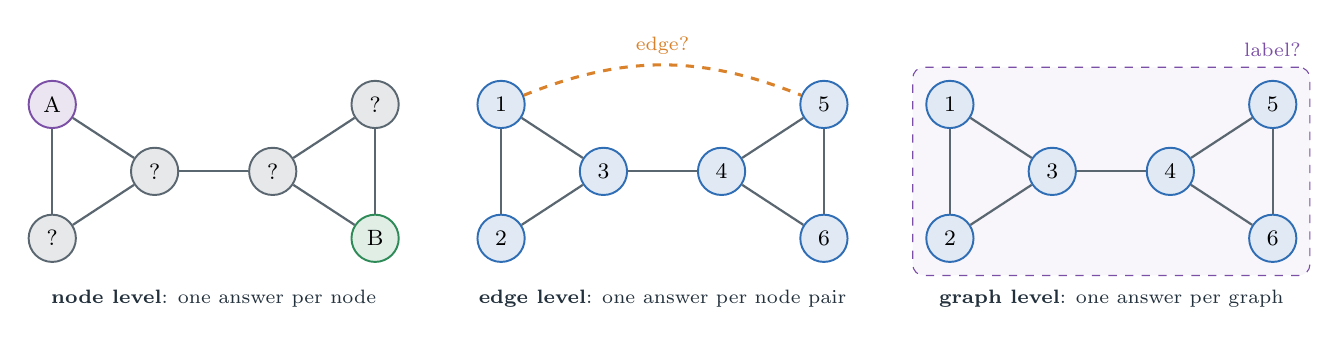
\begin{tikzpicture}
  \begin{scope}[shift={(0,0)}]
    \toycoords
    \foreach \i/\c/\t in {1/cOut/A,2/cTok/?,3/cTok/?,4/cTok/?,5/cTok/?,6/cFfn/B} \node[gnode=\c] (n\i) at (c\i) {\t};
    \toyedges
    \node[note,text=cInk] at (2.05,-1.62) {\textbf{node level}: one answer per node};
  \end{scope}
  \begin{scope}[shift={(5.7,0)}]
    \toygraph
    \draw[cAtt,dashed,line width=1.1pt] (n1) to[bend left=22] node[above,font=\scriptsize,text=cAtt]{edge?} (n5);
    \node[note,text=cInk] at (2.05,-1.62) {\textbf{edge level}: one answer per node pair};
  \end{scope}
  \begin{scope}[shift={(11.4,0)}]
    \toygraph
    \begin{scope}[on background layer]
      \node[draw=cOut,dashed,rounded corners=4pt,fit=(n1)(n2)(n5)(n6),inner sep=1.6mm,fill=cOut!5] (box) {};
    \end{scope}
    \node[note,text=cOut,anchor=south east] at (box.north east) {label?};
    \node[note,text=cInk] at (2.05,-1.62) {\textbf{graph level}: one answer per graph};
  \end{scope}
\end{tikzpicture}

\vspace{-1mm}
{\footnotesize
\renewcommand{\arraystretch}{1.05}
\begin{tabular}{@{}p{21mm}p{45mm}p{45mm}p{45mm}@{}}
\toprule
 & \textbf{Node} & \textbf{Edge (link)} & \textbf{Graph}\\
\midrule
question & what is node $v$? & are $u$ and $v$ related? & what is this whole graph?\\
example & topic of a paper; role of a user & friend suggestion & is this molecule toxic?\\
data & \textbf{one} big graph, few labelled nodes & one graph, some edges hidden & \textbf{many} small graphs, a label each\\
output head & $\hat y_v=\softmax(h_vW)$ & $s_{uv}=\sigma(h_u\cdot h_v)$ & $\hat y_G=\MLP\bigl(\sum_{v\in G}h_v\bigr)$\\
\bottomrule
\end{tabular}}

\vspace{0.5mm}
\begin{columns}[T,onlytextwidth]
\column{0.56\textwidth}
\begin{block}{One encoder, three heads}
\footnotesize
A GNN turns the features $x_v$ into an \key{embedding} $h_v\in\R^{F'}$ per node, a summary of the node
\emph{and its surroundings}. The three tasks differ only in the last step.
\end{block}
\column{0.41\textwidth}
\footnotesize
\vspace{1mm}
This deck trains node classifiers (slides 5--19) and shows the graph-level machinery on slide 14.
Message passing \cite{3} came from graph-level chemistry, GCN \cite{2} from node classification.
\end{columns}
\end{frame}

% ======================================================================= 5
\begin{frame}{Labelled data on a graph: masks instead of separate files}
\begin{columns}[T,onlytextwidth]
\column{0.50\textwidth}
\centering
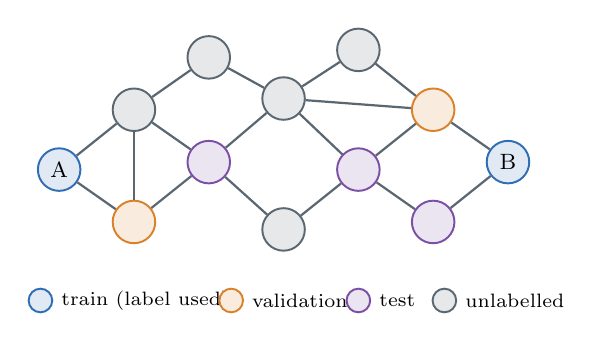
\begin{tikzpicture}[x=9.5mm,y=9.5mm]
  \foreach \n/\x/\y/\c/\t in {a/0/0/cEmb/A,b/1/0.8/cTok/,c/1/-0.7/cAtt/,d/2/0.1/cOut/,e/3/0.95/cTok/,f/3/-0.8/cTok/,
       g/4/0/cOut/,h/5/0.8/cAtt/,i/5/-0.7/cOut/,j/6/0.1/cEmb/B,k/2/1.5/cTok/,l/4/1.6/cTok/}
    \node[gnode=\c,minimum size=5.4mm] (\n) at (\x,\y) {\t};
  \foreach \a/\b in {a/b,a/c,b/c,b/d,c/d,d/e,d/f,e/g,f/g,g/h,g/i,h/j,i/j,e/h,b/k,k/e,e/l,l/h} \draw[gedge] (\a)--(\b);
  \foreach \c/\t/\x in {cEmb/train (label used)/0,cAtt/validation/2.55,cOut/test/4.25,cTok/unlabelled/5.4}
    {\node[gnode=\c,minimum size=3mm] at (\x-0.25,-1.75) {}; \node[anchor=west,font=\scriptsize] at (\x-0.1,-1.75) {\t};}
\end{tikzpicture}

\vspace{1mm}
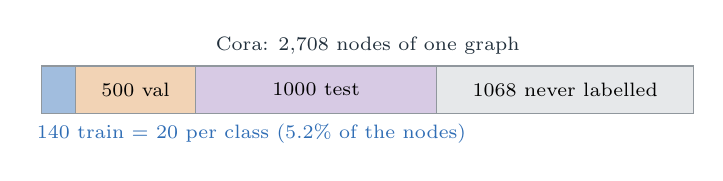
\begin{tikzpicture}[x=0.0306mm,y=1mm,font=\scriptsize]
  \fill[cEmb!45] (0,0) rectangle (140,6); \fill[cAtt!35] (140,0) rectangle (640,6);
  \fill[cOut!30] (640,0) rectangle (1640,6); \fill[cTok!15] (1640,0) rectangle (2708,6);
  \draw[cInk!50] (0,0) rectangle (2708,6); \draw[cInk!50] (140,0)--(140,6) (640,0)--(640,6) (1640,0)--(1640,6);
  \node at (390,3) {500 val}; \node at (1140,3) {1000 test}; \node at (2174,3) {1068 never labelled};
  \node[note,text=cEmb,anchor=west] at (-60,-2.6) {140 train = 20 per class (\coraLabelledPct\% of the nodes)};
  \node[note,text=cInk] at (1354,8.6) {Cora: \coraNodes{} nodes of one graph};
\end{tikzpicture}

\vspace{1mm}
\raggedright\footnotesize
\textbf{Our split}: for each seed, 20 random nodes per class for training, then 500 validation and
1000 test nodes at random from the rest. These are the \emph{sizes} of the Planetoid split \cite{12},
\textbf{not} the fixed public split of \cite{2}. Results depend on the split \cite{13}; we report 10.
\column{0.47\textwidth}
\footnotesize
A \key{label} $y_v$ is the known answer for node $v$ (the topic of a paper). Labels are expensive;
edges and features are cheap.
\begin{block}{Why not split the rows, as for a table?}
\footnotesize
With i.i.d.\ data we cut the table in three and never show test rows to the model.
Here the examples are \emph{connected}: remove the test nodes and the training nodes lose
neighbours. So we keep \textbf{one graph} and split only the \textbf{labels}, with three boolean
\key{masks} over the nodes.
\end{block}
\vspace{-0.5mm}
\begin{itemize}\footnotesize
  \item \key{Transductive} (semi-supervised) learning: the model sees the features and edges of
        \emph{all} nodes while training, test nodes included. Only their labels are hidden.
        Validation labels steer early stopping; test labels give one final number.
  \item The loss averages over the training mask $V_L$ only:
        \vspace{-1.5mm}\[\textstyle \mathcal L=-\frac1{|V_L|}\sum_{v\in V_L}\ln p_v[y_v],\qquad p_v=\softmax(z_v).\]
        \vspace{-5mm}
  \item \key{Inductive} setting: test on nodes or graphs unseen in training \cite{4} (slide 14).
  \item \textbf{Leakage} = a test \emph{label} reaching the model. \texttt{test\_gnn.py} flips all
        non-training labels and checks that training does not change.
\end{itemize}
\end{columns}
\end{frame}

% ======================================================================= 6
\begin{frame}{Node order is arbitrary: permutation equivariance and invariance}
\begin{columns}[T,onlytextwidth]
\column{0.50\textwidth}
\centering
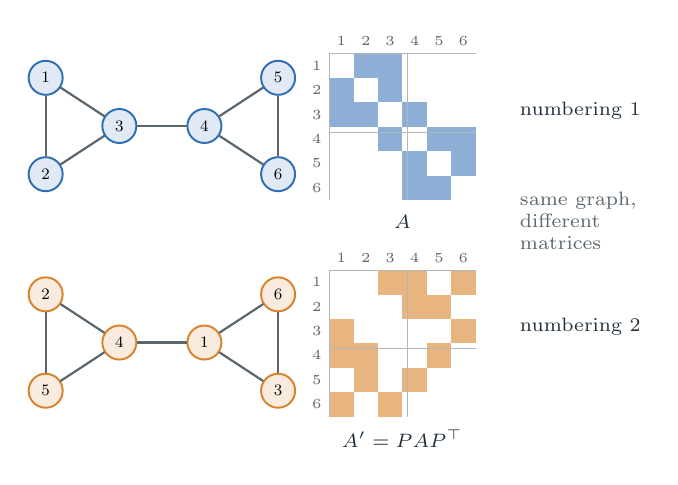
\begin{tikzpicture}
  \begin{scope}[scale=0.72,transform shape]
    \toygraph
  \end{scope}
  \begin{scope}[shift={(3.6,0.92)},x=3.1mm,y=3.1mm]
    \adjgrid{1/2,1/3,2/3,3/4,4/5,4/6,5/6}{cEmb!55}
    \node[note,text=cInk] at (3,-6.9) {$A$};
  \end{scope}
  \begin{scope}[shift={(0,-2.75)}]
    \begin{scope}[scale=0.72,transform shape]
      \toycoords
      \foreach \i/\t in {1/2,2/5,3/4,4/1,5/6,6/3} \node[gnode=cAtt] (n\i) at (c\i) {\t};
      \toyedges
    \end{scope}
    \begin{scope}[shift={(3.6,0.92)},x=3.1mm,y=3.1mm]
      \adjgrid{2/5,2/4,4/5,1/4,1/6,1/3,3/6}{cAtt!60}
      \node[note,text=cInk] at (3,-6.9) {$A'=PAP^\T$};
    \end{scope}
  \end{scope}
  \node[note,text=cInk,anchor=west] at (5.9,0.2) {numbering 1};
  \node[note,text=cInk,anchor=west] at (5.9,-2.55) {numbering 2};
  \node[note,anchor=west,align=left] at (5.9,-1.2) {same graph,\\different\\matrices};
\end{tikzpicture}

\vspace{0.5mm}
\raggedright\footnotesize
The numbers 1..6 are our bookkeeping, not data. A relabelling is a permutation matrix $P$:
$X\to PX$, $A\to PAP^\T$. There are $6!=720$ numberings of this graph, about $10^{8121}$ of Cora.
\column{0.47\textwidth}
\small
\begin{block}{What we must demand of a model $f$}
\footnotesize
\key{Invariance} (one output per graph): same answer, \ $f(PAP^\T,\,PX)=f(A,\,X)$.

\vspace{0.5mm}
\key{Equivariance} (one output per node): the output rows are reordered like the nodes.
\vspace{-1.5mm}\[ F(PAP^\T,\,PX)=P\,F(A,\,X) \]
\vspace{-5mm}
\end{block}
\vspace{-0.5mm}
{\footnotesize\textbf{The layer of slide 8 passes}, since $P^\T P=I$ and an elementwise $\sigma$ commutes with $P$:}
\vspace{-1mm}
\[ \sigma\bigl((P\Ah P^\T)(PX)W\bigr)=P\,\sigma(\Ah XW). \]
\vspace{-5mm}
\begin{block}{Measured on the example (\texttt{walkthrough.py}, part 4)}
\footnotesize
\renewcommand{\arraystretch}{1.1}
\begin{tabular}{@{}p{33mm}ll@{}}
 & numbering 1 & numbering 2\\
\midrule
GCN layer, old node 4 & $(.211,\,.202)$ & $(.211,\,.202)$\\
GCN layer, sum of rows & $(1.199,\,1.003)$ & $(1.199,\,1.003)$\\
linear layer on flat $[A,X]$ & $2.061$ & {\color{cBad}$-0.680$}\\
\end{tabular}

\vspace{0.5mm}
$F(PAP^\T,PX)$ and $P\,F(A,X)$ agree exactly.
\end{block}
\end{columns}
\end{frame}

% ======================================================================= 7
\begin{frame}{Message passing: aggregate the neighbours, then update}
\begin{columns}[T,onlytextwidth]
\column{0.50\textwidth}
\centering
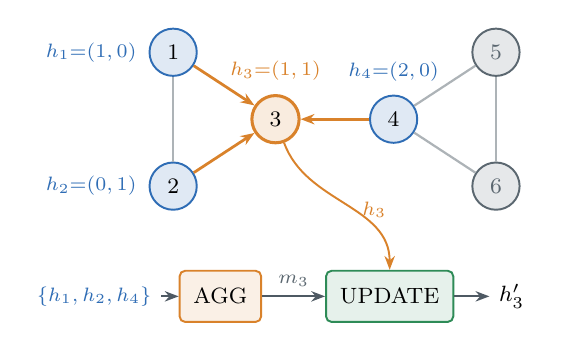
\begin{tikzpicture}
  \toycoords
  \foreach \i in {1,2,4} \node[gnode] (n\i) at (c\i) {\i};
  \foreach \i in {5,6} \node[gnode=cTok,text=cTok] (n\i) at (c\i) {\i};
  \node[gnode=cAtt,line width=1.1pt] (n3) at (c3) {3};
  \foreach \a/\b in {1/2,4/5,4/6,5/6} \draw[gedge,cTok!50] (n\a)--(n\b);
  \foreach \i in {1,2,4} \draw[msg] (n\i)--(n3);
  \node[note,text=cEmb,left=0.3mm of n1] {$h_1{=}(1,0)$}; \node[note,text=cEmb,left=0.3mm of n2] {$h_2{=}(0,1)$};
  \node[note,text=cEmb,above=0.5mm of n4] {$h_4{=}(2,0)$}; \node[note,text=cAtt,above=0.5mm of n3] {$h_3{=}(1,1)$};
  \node[stage=cAtt,minimum height=6.5mm,font=\footnotesize] (agg) at (0.6,-2.25) {$\AGG$};
  \node[stage=cFfn,minimum height=6.5mm,font=\footnotesize] (upd) at (2.75,-2.25) {$\UPD$};
  \node[font=\footnotesize] (out) at (4.3,-2.25) {$h_3'$};
  \draw[flow] (agg)-- node[above,note]{$m_3$} (upd); \draw[flow] (upd)--(out);
  \draw[flow,cAtt] (n3) to[out=-70,in=90] node[right,note,pos=0.55,text=cAtt]{$h_3$} (upd.north);
  \node[note,text=cEmb,anchor=east] (set) at (-0.15,-2.25) {$\{h_1,h_2,h_4\}$};
  \draw[flow] (set)--(agg);
\end{tikzpicture}

\vspace{-0.5mm}
\begin{block}{One message-passing layer \cite{3}}
\vspace{-2.5mm}
\[
  h_v' \;=\; \UPD\Bigl(h_v,\ \AGG\bigl(\{\,h_u : u\in\N(v)\,\}\bigr)\Bigr)
\]
\vspace{-4mm}
\end{block}
{\footnotesize
\renewcommand{\arraystretch}{1.2}
\begin{tabular}{@{}llll@{}}
\toprule
$\AGG$ & at node 3 & all nodes at once & cannot tell apart\\
\midrule
sum & $(3,\,1)$ & $AH$ & keeps counts (slide 13)\\
mean & $(1,\,\tfrac13)$ & $D^{-1}AH$ & $\{a,b\}$ and $\{a,a,b,b\}$\\
max & $(2,\,1)$ & elementwise & $\{a,b\}$ and $\{a,b,b\}$\\
\bottomrule
\end{tabular}}
\column{0.47\textwidth}
\footnotesize
\begin{itemize}
  \item Each node holds a vector $h_v$, starting from its features: $h_v^{(0)}=x_v$.
  \item \key{Aggregate}: collect the neighbours' vectors into one \key{message} $m_v$. The neighbours
        form a \emph{set}: no order, any size. So $\AGG$ must ignore order and accept any number of
        inputs: sum, mean, max \cite{9}.
  \item \key{Update}: combine the message with the node's own vector, using \textbf{trainable weights}
        and a nonlinearity, e.g.\ $h_v'=\ReLU(h_vW_1+m_vW_2)$.
  \item The \textbf{same weights at every node}: the number of parameters does not depend on the
        size of the graph, and a trained layer runs on any graph.
\end{itemize}
\vspace{-1mm}
\begin{block}{Why this is the right shape}
\footnotesize
Order-free aggregation plus shared weights gives permutation equivariance (slide 6) by construction.
In a CNN the ``neighbours'' are the pixels under the filter; they have a fixed order, so each gets
its own weight. On a graph they have none, so they are pooled first.
\end{block}
{\footnotesize GCN, GraphSAGE, GAT and GIN (slides 8, 12, 13) differ only in $\AGG$ and $\UPD$.}
\end{columns}
\end{frame}

% ======================================================================= 8
\begin{frame}{The GCN layer: one matrix equation}
\begin{columns}[T,onlytextwidth]
\column{0.50\textwidth}
\begin{block}{Graph convolutional layer (Kipf \& Welling \cite{2})}
\vspace{-2.5mm}
\[
  H'=\sigma\bigl(\Ah\,H\,W\bigr),\quad\ \Ah=\Dt^{-1/2}\,\At\,\Dt^{-1/2},\quad\ \At=A+I
\]
\vspace{-4.5mm}

{\footnotesize $H\in\R^{n\times F}$: one row per node. \ $W\in\R^{F\times F'}$: the trainable weights.
\ $\Dt=\diag(\dt)$, $\dt_v=d_v+1$. \ $\sigma$: ReLU.}
\end{block}
\centering
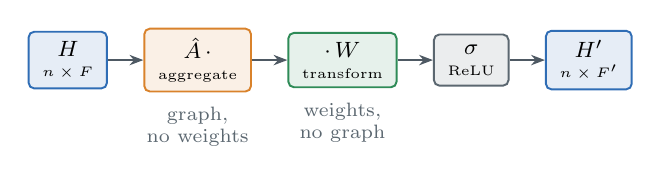
\begin{tikzpicture}[node distance=4.5mm,font=\footnotesize]
  \node[stage=cEmb,minimum height=6.5mm,font=\footnotesize] (h) {$H$\\[-2pt]{\tiny $n\times F$}};
  \node[stage=cAtt,minimum height=6.5mm,font=\footnotesize,right=of h] (a) {$\Ah\,\cdot$\\[-2pt]{\tiny aggregate}};
  \node[stage=cFfn,minimum height=6.5mm,font=\footnotesize,right=of a] (w) {$\cdot\,W$\\[-2pt]{\tiny transform}};
  \node[stage=cTok,minimum height=6.5mm,font=\footnotesize,right=of w] (s) {$\sigma$\\[-2pt]{\tiny ReLU}};
  \node[stage=cEmb,minimum height=6.5mm,font=\footnotesize,right=of s] (o) {$H'$\\[-2pt]{\tiny $n\times F'$}};
  \draw[flow] (h)--(a); \draw[flow] (a)--(w); \draw[flow] (w)--(s); \draw[flow] (s)--(o);
  \node[note,below=0.6mm of a] {graph,\\no weights};
  \node[note,below=0.6mm of w] {weights,\\no graph};
\end{tikzpicture}

\vspace{0.5mm}
\raggedright\small
\textbf{The same equation, one node at a time} ($h_v$ = row $v$ of $H$):
\vspace{-1.5mm}
\[
  h_v'=\sigma\Bigl(\sum_{u\,\in\,\N(v)\cup\{v\}}\frac{1}{\sqrt{\dt_v\,\dt_u}}\;h_u\,W\Bigr)
\]
\vspace{-3.5mm}

{\footnotesize Message passing with a \textbf{weighted sum} as $\AGG$ and ``times $W$, then $\sigma$'' as $\UPD$.
\textbf{Parameters}: $F\!\cdot\!F'$ per layer, whatever $n$ is. Our Cora model $1433\to16\to7$ with biases has
$1433\cdot16+16+16\cdot7+7=\num{23{,}063}$.}
\column{0.47\textwidth}
\small
\key{Why add self-loops?} \ $(AH)_v$ sums the neighbours only: a node's \emph{own} features would
vanish from its update. With $\At=A+I$ every node is also its own neighbour.

\vspace{1.5mm}
\key{Why normalise?} \ $(\At H)_v$ is a sum over $\dt_v$ nodes. A paper with 168 links would get
a vector roughly 40 times longer than a typical one, and every layer multiplies again:
\begin{itemize}\footnotesize
  \item on the example graph the largest eigenvalue of $\At$ is $3.41$, so $k$ layers can scale
        features by $3.41^k$;
  \item all eigenvalues of $\Ah$ lie in $(-1,\,1]$. Nothing explodes.
\end{itemize}

\vspace{0.5mm}
\key{Why $\Dt^{-1/2}\cdots\Dt^{-1/2}$, not the mean $\Dt^{-1}\At$?}
\begin{itemize}\footnotesize
  \item The mean weights each neighbour by $1/\dt_v$. The symmetric form uses $1/\sqrt{\dt_v\dt_u}$:
        a message from a hub $u$ (large $\dt_u$) counts for less.
  \item $\Ah$ stays \textbf{symmetric}: real eigenvalues, orthogonal eigenvectors (slide 11).
        Both work in practice; GraphSAGE uses the mean (slide 12).
\end{itemize}
\vspace{0.5mm}
{\footnotesize \textbf{Origin}: \cite{2} derives the layer as a first-order approximation of a spectral filter on
the graph Laplacian $L=I-D^{-1/2}AD^{-1/2}$. It can be used without that derivation.}
\end{columns}
\end{frame}

% ======================================================================= 9
\begin{frame}{A GCN layer by hand on the example graph}
\begin{columns}[T,onlytextwidth]
\column{0.53\textwidth}
\small
\textbf{1. Self-loops and degrees.} \ $\At=A+I$, \ $\dt=(3,3,4,4,3,3)$.

\vspace{1mm}
\textbf{2. Normalise.} \ $\Ah_{vu}=1/\sqrt{\dt_v\dt_u}$ wherever $\At_{vu}=1$:
{\scriptsize
\[
 \Ah=\begin{bmatrix}
 .333&.333&.289&0&0&0\\ .333&.333&.289&0&0&0\\ \mathbf{.289}&\mathbf{.289}&\mathbf{.250}&\mathbf{.250}&0&0\\
 0&0&.250&.250&.289&.289\\ 0&0&0&.289&.333&.333\\ 0&0&0&.289&.333&.333
 \end{bmatrix}
 \qquad
 \begin{aligned}
  \tfrac13&=\tfrac1{\sqrt{3\cdot3}}\\[1pt] .289&=\tfrac1{\sqrt{3\cdot4}}\\[1pt] \tfrac14&=\tfrac1{\sqrt{4\cdot4}}
 \end{aligned}
\]}
\vspace{-2mm}

\textbf{3. Aggregate}: $S=\Ah X$. \ \textbf{4. Transform}: $SW$. \ \textbf{5. ReLU}.
{\scriptsize
\[
 \underbrace{\begin{bmatrix}.622&.622\\.622&.622\\\mathbf{1.039}&\mathbf{.539}\\1.039&.827\\.911&.667\\.911&.667\end{bmatrix}}_{S=\Ah X}
 \underbrace{\begin{bmatrix}1&-1\\-1&1.5\end{bmatrix}}_{W}
 =\begin{bmatrix}0&.311\\0&.311\\\mathbf{.500}&\mathbf{-.231}\\.211&.202\\.244&.089\\.244&.089\end{bmatrix}
 \ \xrightarrow{\ \ReLU\ }\
 \underbrace{\begin{bmatrix}0&.311\\0&.311\\\mathbf{.500}&\mathbf{0}\\.211&.202\\.244&.089\\.244&.089\end{bmatrix}}_{H'}
\]}
\column{0.44\textwidth}
\centering
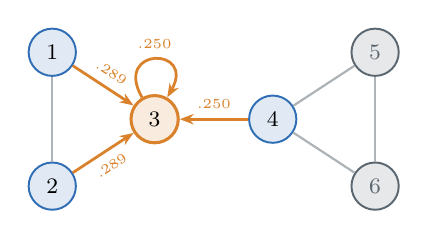
\begin{tikzpicture}
  \toycoords
  \foreach \i in {1,2,4} \node[gnode] (n\i) at (c\i) {\i};
  \foreach \i in {5,6} \node[gnode=cTok,text=cTok] (n\i) at (c\i) {\i};
  \node[gnode=cAtt,line width=1.1pt] (n3) at (c3) {3};
  \foreach \a/\b in {1/2,4/5,4/6,5/6} \draw[gedge,cTok!50] (n\a)--(n\b);
  \draw[msg] (n1)-- node[above,sloped,font=\tiny,text=cAtt]{.289} (n3);
  \draw[msg] (n2)-- node[below,sloped,font=\tiny,text=cAtt]{.289} (n3);
  \draw[msg] (n4)-- node[above,font=\tiny,text=cAtt]{.250} (n3);
  \draw[msg] (n3) to[out=120,in=60,looseness=6] node[above,font=\tiny,text=cAtt]{.250} (n3);
\end{tikzpicture}

\vspace{-1mm}
\raggedright
\begin{block}{Row 3 in detail (bold; \texttt{walkthrough.py}, part 3)}
\footnotesize
Node 3 has neighbours 1, 2, 4 and itself:
\vspace{-1.5mm}
\begin{align*}
 s_3&=\tfrac14x_3+\tfrac1{\sqrt{12}}x_1+\tfrac1{\sqrt{12}}x_2+\tfrac14x_4\\
    &=\tfrac14(1,1)+.289\,(1,0)+.289\,(0,1)+\tfrac14(2,0)\\
    &=(\num{1.039},\ \num{0.539})\\[2pt]
 s_3W&=(1.039-.539,\ -1.039+1.5\cdot.539)=(.500,\,-.231)\\
 h_3'&=\ReLU(s_3W)=(\num{0.500},\ \num{0})
\end{align*}
\vspace{-5mm}
\end{block}
\begin{itemize}\footnotesize
  \item Nodes 1 and 2 have the same neighbourhood $\{1,2,3\}$, so they get \textbf{the same output}
        although $x_1\neq x_2$. Likewise 5 and 6.
  \item With the plain mean $\Dt^{-1}\At$, $s_3=(1,\,0.5)$; unnormalised, $(4,\,2)$.
\end{itemize}
\end{columns}
\end{frame}

% ====================================================================== 10
\begin{frame}{Stacking layers: $k$ layers see $k$ hops}
\begin{columns}[T,onlytextwidth]
\column{0.50\textwidth}
\centering
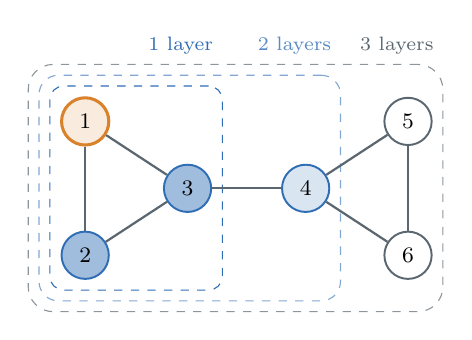
\begin{tikzpicture}
  \toycoords
  \node[gnode=cAtt,line width=1.1pt] (n1) at (c1) {1};
  \node[gnode=cEmb,fill=cEmb!45] (n2) at (c2) {2}; \node[gnode=cEmb,fill=cEmb!45] (n3) at (c3) {3};
  \node[gnode=cEmb,fill=cEmb!18] (n4) at (c4) {4};
  \node[gnode=cTok,fill=white] (n5) at (c5) {5}; \node[gnode=cTok,fill=white] (n6) at (c6) {6};
  \toyedges
  \begin{scope}[on background layer]
    \node[draw=cEmb,dashed,rounded corners=5pt,fit=(n1)(n2)(n3),inner sep=1.3mm] (r1) {};
    \node[draw=cEmb!60,dashed,rounded corners=7pt,fit=(r1)(n4),inner sep=1.3mm] (r2) {};
    \node[draw=cTok!70,dashed,rounded corners=9pt,fit=(r2)(n5)(n6),inner sep=1.3mm] (r3) {};
  \end{scope}
  \node[note,text=cEmb,anchor=south east] at (r1.east|-r3.north) {1 layer};
  \node[note,text=cEmb!80,anchor=south east] at (r2.east|-r3.north) {2 layers};
  \node[note,anchor=south east] at (r3.north east) {3 layers};
\end{tikzpicture}

\vspace{0.5mm}
{\footnotesize\color{cTok}Which inputs can influence node 1 (orange)? Its \key{receptive field} grows by one hop per layer.}

\vspace{1mm}
\raggedright\small
A 2-layer GCN (the model we train):
\vspace{-1.5mm}
\[
  Z=\Ah\;\ReLU\bigl(\Ah XW^{1}\bigr)\,W^{2},\qquad \hat y_v=\softmax(z_v)
\]
\vspace{-5mm}
\begin{itemize}\footnotesize
  \item Layer 1 mixes each node with its neighbours. Layer 2 mixes those mixtures: now neighbours
        of neighbours contribute. Each layer has its own $W^\ell$; $\Ah$ is shared.
  \item In general $h_v^{(k)}$ depends on $x_u$ only if $u$ is within $k$ hops, i.e.\ $(\At^k)_{vu}\neq0$.
        Example: $(\Ah^2)_{1\cdot}=(.31,\ .31,\ .26,\ .07,\ 0,\ 0)$: node 4 has arrived, nodes 5, 6 not yet.
\end{itemize}
\column{0.47\textwidth}
\centering
\begin{tikzpicture}
\begin{semilogyaxis}[width=7.6cm,height=4.6cm,xmin=0,xmax=8,ymin=0.8,ymax=4000,
  xlabel={number of hops $k$ (= layers)},ylabel={nodes within $k$ hops},label style={font=\scriptsize},
  tick label style={font=\tiny},axis lines=left,ymajorgrids,grid style={cInk!10},log ticks with fixed point,
  ytick={1,10,100,1000},xtick={0,...,8},
  legend style={font=\scriptsize,draw=none,fill=none,at={(0.98,0.05)},anchor=south east},legend cell align=left,
  every axis plot/.append style={line width=1.1pt,mark size=1.5pt}]
  \addplot[cEmb,mark=*] table[x=k,y=mean]{generated/hops.dat}; \addlegendentry{mean over nodes}
  \addplot[cAtt,mark=square*,dashed] table[x=k,y=median]{generated/hops.dat}; \addlegendentry{median}
  \draw[cTok,densely dotted] (axis cs:0,2708) -- (axis cs:8,2708);
  \node[font=\tiny,text=cTok,anchor=south west] at (axis cs:0.1,2708) {all 2{,}708 nodes};
\end{semilogyaxis}
\end{tikzpicture}

\vspace{-0.5mm}
{\scriptsize\color{cTok}Measured on Cora by \texttt{experiments.py} (the node itself counts).}

\vspace{1mm}
\raggedright\footnotesize
\begin{itemize}
  \item \textbf{Neighbourhoods grow fast.} On Cora a node reaches \hopOneMean{} nodes on average in 1 hop,
        \hopTwoMean{} in 2, \hopFourMean{} in 4 (\hopFourPct\% of the graph) and \hopEightPct\% in 8.
  \item So 2 layers already pool information from dozens of papers. That is why shallow GNNs
        work, unlike CNNs or transformers where depth keeps paying.
  \item \textbf{The cost of depth}: with many layers every node's receptive field is nearly the whole
        graph, and all nodes start to compute the same average. Next slide.
\end{itemize}
\end{columns}
\end{frame}

% ====================================================================== 11
\begin{frame}{Depth has a price: over-smoothing}
\begin{columns}[T,onlytextwidth]
\column{0.49\textwidth}
\centering
\begin{tikzpicture}
\begin{axis}[width=8.3cm,height=4.0cm,xmin=0.7,xmax=8.3,ymin=0,ymax=105,
  xlabel={number of GCN layers},ylabel={accuracy (\%)},label style={font=\scriptsize},tick label style={font=\tiny},
  axis lines=left,ymajorgrids,grid style={cInk!10},xtick={1,...,8},ytick={0,20,40,60,80,100},
  legend style={font=\scriptsize,draw=none,fill=white,fill opacity=0.8,text opacity=1,at={(0.02,0.03)},anchor=south west},legend cell align=left,
  every axis plot/.append style={line width=1.1pt,mark size=1.5pt}]
  \addplot[cEmb,mark=*,error bars/.cd,y dir=both,y explicit] table[x=L,y=mean,y error=std]{generated/depth.dat};
  \addlegendentry{GCN, test}
  \addplot[cEmb,dashed,mark=o,line width=0.8pt] table[x=L,y=train]{generated/depth.dat};
  \addlegendentry{GCN, train}
  \addplot[cFfn,mark=square*,error bars/.cd,y dir=both,y explicit] table[x=L,y=res_mean,y error=res_std]{generated/depth.dat};
  \addlegendentry{GCN + skip, test}
\end{axis}
\end{tikzpicture}

\vspace{-0.5mm}
{\scriptsize\color{cTok}Measured: Cora, mean $\pm$ std over \depthSeeds{} splits; train = the 140 labelled nodes.}

\vspace{1mm}
\raggedright\footnotesize
\begin{itemize}
  \item \textbf{Two layers are best}: \depthOne\% with 1 layer, \textbf{\depthTwo\%} with 2, \depthFour\% with 4,
        \depthEight\% with 8.
  \item \textbf{Honest reading}: from 5 layers on, the plain GCN does not even fit its 140 training labels
        (\depthTrainFive\% at 5 layers, \depthTrainEight\% at 8). It fails to \emph{train}, not only to
        generalise. Over-smoothing is one cause; dropout before every layer and shrinking gradients
        are others. We did not separate them.
  \item \key{Skip connections} $H^{\ell}=\sigma(\Ah H^{\ell-1}W^\ell)+H^{\ell-1}$ keep each node's own signal.
        They repair training (\depthResEight\% test at 8 layers), but depth still does not \emph{help} here.
\end{itemize}
\column{0.48\textwidth}
\footnotesize
\key{Over-smoothing} \cite{10,11}: every layer averages over neighbours. Average often enough and
all nodes look alike.
\begin{block}{Why: powers of $\Ah$}
\footnotesize
$\Ah$ is symmetric: $\Ah=\sum_i\lambda_iu_iu_i^\T$, with $1=\lambda_1>|\lambda_2|\ge\dots$ on a connected graph.
Ignoring $W$ and $\sigma$, $k$ layers compute
\vspace{-1.5mm}
\[
 \Ah^kX=\sum_i\lambda_i^k\,u_i\,(u_i^\T X)\ \xrightarrow{\;k\to\infty\;}\ u_1\,(u_1^\T X),\qquad (u_1)_v\propto\sqrt{\dt_v}.
\]
\vspace{-4.5mm}

Every row becomes a multiple of the \emph{same} vector: what a node knew about itself is gone, only its
degree is left.
\end{block}
\centering
\begin{tikzpicture}
\begin{axis}[width=7.9cm,height=3.2cm,xmin=0,xmax=64,ymin=0,ymax=1,
  xlabel={propagation steps $k$ in $\Ah^kX$},ylabel={cosine similarity},label style={font=\scriptsize},
  tick label style={font=\tiny},axis lines=left,ymajorgrids,grid style={cInk!10},xtick={0,8,16,24,32,48,64},
  every axis plot/.append style={line width=1.1pt,mark size=1.4pt}]
  \addplot[cAtt,mark=*] table[x=k,y=cos]{generated/smooth.dat};
\end{axis}
\end{tikzpicture}

\vspace{-1mm}
{\scriptsize\color{cTok}Measured on Cora: mean cosine similarity over 5{,}000 random node pairs.}

\vspace{0.5mm}
\raggedright\footnotesize
Random pairs start near-orthogonal (\smoothZero); \smoothTwo{} after 2 steps, \smoothEight{} after 8, \smoothSixtyFour{} after 64.
A little smoothing makes same-topic papers alike and helps. A lot makes \emph{all} papers alike.
\end{columns}
\end{frame}

% ====================================================================== 12
\begin{frame}{Variants I: GraphSAGE and graph attention (GAT)}
\begin{columns}[T,onlytextwidth]
\column{0.49\textwidth}
\begin{block}{GraphSAGE \cite{4}: mean, then concatenate}
\vspace{-2.5mm}
\[
 h_v'=\sigma\bigl(\bigl[\,h_v\ \|\ \bar h_{\N(v)}\bigr]W\bigr)
     =\sigma\bigl(h_vW_{\text{self}}+\bar h_{\N(v)}W_{\text{neigh}}\bigr)
\]
\vspace{-4mm}

\footnotesize
\begin{itemize}
  \item $\bar h_{\N(v)}$: mean of the neighbours' vectors; $\|$: concatenation. The node's own vector
        gets \textbf{its own weights}.
  \item For large graphs: \emph{sample} a few neighbours per node, train on mini-batches. The rule
        also applies to nodes never seen in training (inductive).
\end{itemize}
\end{block}
\vspace{-0.5mm}
\begin{block}{GAT \cite{5}: learn the weight of each neighbour}
\vspace{-3mm}\footnotesize
\begin{align*}
 e_{vu}&=\LeakyReLU\bigl(a_{\text{dst}}\!\cdot\!(h_vW)+a_{\text{src}}\!\cdot\!(h_uW)\bigr)\\[-2pt]
 \alpha_{vu}&=\softmax_{u}(e_{vu}),\qquad h_v'=\sigma\bigl(\textstyle\sum_{u}\alpha_{vu}\,h_uW\bigr)
\end{align*}
\vspace{-4.5mm}

\footnotesize
\begin{itemize}
  \item $u$ runs over $\N(v)\cup\{v\}$. GCN's fixed $1/\sqrt{\dt_v\dt_u}$ becomes an \key{attention
        coefficient} $\alpha_{vu}$ computed from the two nodes' features; $W$, $a_{\text{dst}}$, $a_{\text{src}}$ are trained. Several \textbf{heads} run in
        parallel and are concatenated (8 heads of 8 units in \cite{5} and here).
\end{itemize}
\end{block}
\column{0.48\textwidth}
\centering
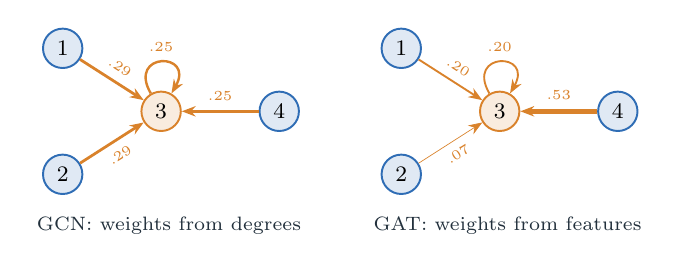
\begin{tikzpicture}[font=\tiny]
  \foreach \sx/\ttl/\va/\vb/\vc/\vd/\la/\lb/\lc/\ld in
     {0/{GCN: weights from degrees}/1.0/1.0/0.87/0.87/.29/.29/.25/.25,
      4.3/{GAT: weights from features}/0.68/0.25/0.68/1.85/.20/.07/.20/.53} {
    \begin{scope}[shift={(\sx,0)}]
      \node[gnode,minimum size=5mm] (a) at (0,0.8) {1}; \node[gnode,minimum size=5mm] (b) at (0,-0.8) {2};
      \node[gnode=cAtt,minimum size=5mm] (c) at (1.25,0) {3}; \node[gnode,minimum size=5mm] (d) at (2.75,0) {4};
      \draw[cAtt,->,line width=\va pt] (a)-- node[above,sloped,text=cAtt]{\la} (c);
      \draw[cAtt,->,line width=\vb pt] (b)-- node[below,sloped,text=cAtt]{\lb} (c);
      \draw[cAtt,->,line width=\vd pt] (d)-- node[above,text=cAtt]{\ld} (c);
      \draw[cAtt,->,line width=\vc pt] (c) to[out=120,in=60,looseness=6] node[above,text=cAtt]{\lc} (c);
      \node[note,text=cInk] at (1.35,-1.45) {\ttl};
    \end{scope}}
\end{tikzpicture}

\vspace{-0.5mm}
{\scriptsize\color{cTok}Node 3 of the example. Right: $W{=}I$, $a_{\text{dst}}{=}0$, $a_{\text{src}}{=}(1,0)$, scores $(1,0,1,2)$. Illustrative, not trained.}

\vspace{1mm}
\raggedright
{\footnotesize
\begin{tabular}{@{}lrrr@{}}
\toprule
Cora, 2 layers & parameters & s / run & test accuracy\\
\midrule
GCN (16 hidden units) & \coraGcnParams & \timeGcn & \coraGcnMean{} $\pm$ \coraGcnStd\,\%\\
GraphSAGE-mean (16) & \coraSageParams & \timeSage & \coraSageMean{} $\pm$ \coraSageStd\,\%\\
GAT ($8\times8$) & \coraGatParams & \timeGat & \coraGatMean{} $\pm$ \coraGatStd\,\%\\
\bottomrule
\multicolumn{4}{@{}l}{\scriptsize\color{cTok}Measured, full-batch; \coraSeeds{} splits (GAT: first \coraGatSeeds). See slide 19.}
\end{tabular}}

\vspace{0.5mm}
\vspace{-0.5mm}
\begin{block}{Remark: a transformer is a GNN on the complete graph}
\footnotesize
Self-attention \cite{18}: $h_v'=\sum_u\alpha_{vu}\,h_uW$, $\alpha_{vu}=\softmax_u(q_v\!\cdot\!k_u/\sqrt d)$ over \emph{all}
tokens $u$. Everyone is everyone's neighbour; order comes from positional encodings, not edges.
\end{block}
\end{columns}
\end{frame}

% ====================================================================== 13
\begin{frame}{Variants II: GIN, and what message passing cannot see}
\begin{columns}[T,onlytextwidth]
\column{0.49\textwidth}
\centering
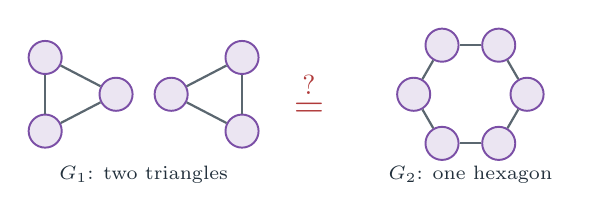
\begin{tikzpicture}
  \begin{scope}[yscale=0.85]
    \foreach \n/\x/\y in {a/0/0.55,b/0/-0.55,c/0.9/0,d/1.6/0,e/2.5/0.55,f/2.5/-0.55} \node[gnode=cOut,minimum size=4.2mm] (\n) at (\x,\y) {};
    \foreach \a/\b in {a/b,a/c,b/c,d/e,d/f,e/f} \draw[gedge] (\a)--(\b);
    \node[note,text=cInk] at (1.25,-1.2) {$G_1$: two triangles};
  \end{scope}
  \begin{scope}[shift={(5.4,0)}]
    \foreach \i in {0,...,5} \node[gnode=cOut,minimum size=4.2mm] (h\i) at ({60*\i}:0.72) {};
    \foreach \i [evaluate=\i as \j using {int(mod(\i+1,6))}] in {0,...,5} \draw[gedge] (h\i)--(h\j);
    \node[note,text=cInk] at (0,-1.02) {$G_2$: one hexagon};
  \end{scope}
  \node[font=\Large,text=cBad] at (3.35,0) {$\overset{?}{=}$};
\end{tikzpicture}

\vspace{0.5mm}
\raggedright\footnotesize
\key{Weisfeiler--Leman (1-WL) test} \cite{7}: can two graphs be told apart? Give every node the same
colour, then repeatedly recolour each node by its own colour and the \emph{multiset} $\{\!\{\cdot\}\!\}$
(a set with repeats) of its neighbours' colours:
\vspace{-1.5mm}
\[
 c_v\ \leftarrow\ \operatorname{hash}\bigl(c_v,\ \{\!\{\,c_u:u\in\N(v)\,\}\!\}\bigr).
\]
\vspace{-5mm}

Different final colour counts prove the graphs different.
\textbf{This is message passing} with $\AGG$ = ``the multiset'' and $\UPD$ = hash. Hence:
\vspace{-0.5mm}
\begin{block}{Theorem (Xu et al.\ \cite{6}, Morris et al.\ \cite{8})}
\footnotesize
A message-passing GNN can distinguish two graphs \emph{at most} when 1-WL can. It reaches that
bound if $\AGG$ and $\UPD$ are injective (lose no information).
\end{block}
\textbf{$G_1$ vs $G_2$ defeats 1-WL}: in both, every node has two neighbours, each with two
neighbours, and so on. All nodes keep one colour, yet $G_1$ has 2 triangles and $G_2$ none.
\column{0.48\textwidth}
\begin{block}{GIN, the graph isomorphism network \cite{6}}
\vspace{-2.5mm}
\[
 h_v'=\MLP\Bigl((1+\epsilon)\,h_v+\sum_{u\in\N(v)}h_u\Bigr)
\]
\vspace{-4mm}

\footnotesize
\textbf{Sum}: it keeps what mean and max discard (slide 7), how \emph{many} neighbours of each kind.
\textbf{MLP}: one linear layer cannot represent every injective update.
With both, GIN is exactly as discriminating as 1-WL.
\end{block}
\vspace{-0.5mm}
\begin{block}{Measured (\texttt{walkthrough.py}, part 8)}
\footnotesize
Random 3-layer GIN, all node features 1, sum readout:

\vspace{0.5mm}
\begin{tabular}{@{}ll@{}}
$G_1$ (two triangles): & $(0.999,\ 0.932,\ 0.032,\ 1.432)$\\
$G_2$ (hexagon): & $(0.999,\ 0.932,\ 0.032,\ 1.432)$
\end{tabular}

\vspace{0.5mm}
Identical for \emph{any} weights: this model cannot count triangles.
\end{block}
\footnotesize
\begin{itemize}\footnotesize
  \item \textbf{In practice} the limit bites when nodes lack distinguishing features. With rich features,
        as in Cora, it rarely matters: GCN is weaker than GIN in theory and does well there.
  \item Remedies: node ids, positional encodings, higher-order networks \cite{8}.
\end{itemize}
\end{columns}
\end{frame}

% ====================================================================== 14
\begin{frame}{Graph-level prediction: readout and batching}
\centering
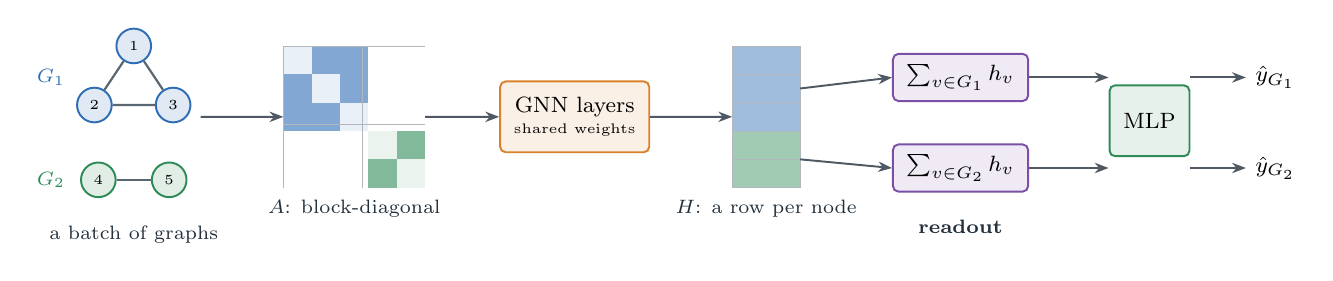
\begin{tikzpicture}[font=\footnotesize]
  % two input graphs
  \node[gnode=cEmb,minimum size=4.4mm] (a1) at (0,0.95) {\tiny1}; \node[gnode=cEmb,minimum size=4.4mm] (a2) at (-0.5,0.2) {\tiny2};
  \node[gnode=cEmb,minimum size=4.4mm] (a3) at (0.5,0.2) {\tiny3};
  \draw[gedge] (a1)--(a2)--(a3)--(a1);
  \node[gnode=cFfn,minimum size=4.4mm] (b1) at (-0.45,-0.75) {\tiny4}; \node[gnode=cFfn,minimum size=4.4mm] (b2) at (0.45,-0.75) {\tiny5};
  \draw[gedge] (b1)--(b2);
  \node[note,text=cEmb,anchor=east] at (-0.75,0.55) {$G_1$}; \node[note,text=cFfn,anchor=east] at (-0.75,-0.75) {$G_2$};
  % block diagonal adjacency
  \begin{scope}[shift={(1.9,0.95)},x=3.6mm,y=3.6mm]
    \fill[cEmb!10] (0,0) rectangle (3,-3); \fill[cFfn!10] (3,-3) rectangle (5,-5);
    \foreach \r/\c in {1/2,1/3,2/3} {\fill[cEmb!60] (\c-1,-\r+1) rectangle ++(1,-1); \fill[cEmb!60] (\r-1,-\c+1) rectangle ++(1,-1);}
    \fill[cFfn!60] (4,-3) rectangle ++(1,-1); \fill[cFfn!60] (3,-4) rectangle ++(1,-1);
    \draw[cInk!35,line width=0.3pt] (0,0) grid (5,-5);
    \node[note,text=cInk] at (2.5,-5.75) {$A$: block-diagonal};
    \coordinate (Aeast) at (5,-2.5); \coordinate (Awest) at (0,-2.5);
  \end{scope}
  \node[stage=cAtt,minimum height=9mm,font=\footnotesize] (gnn) at (5.6,0.05) {GNN layers\\[-2pt]{\tiny shared weights}};
  % node embeddings
  \begin{scope}[shift={(7.6,0.95)},x=3.6mm,y=3.6mm]
    \foreach \r in {1,2,3} \fill[cEmb!45] (0,-\r+1) rectangle ++(2.4,-1);
    \foreach \r in {4,5} \fill[cFfn!45] (0,-\r+1) rectangle ++(2.4,-1);
    \draw[cInk!35,line width=0.3pt] (0,0) rectangle (2.4,-5); \foreach \r in {1,...,4} \draw[cInk!35,line width=0.3pt] (0,-\r)--(2.4,-\r);
    \node[note,text=cInk] at (1.2,-5.75) {$H$: a row per node};
    \coordinate (Hwest) at (0,-2.5); \coordinate (Heast) at (2.4,-2.5);
    \coordinate (Htop) at (2.4,-1.5); \coordinate (Hbot) at (2.4,-4);
  \end{scope}
  \node[stage=cOut,minimum height=6mm,font=\footnotesize] (r1) at (10.5,0.55) {$\sum_{v\in G_1}h_v$};
  \node[stage=cOut,minimum height=6mm,font=\footnotesize] (r2) at (10.5,-0.6) {$\sum_{v\in G_2}h_v$};
  \node[stage=cFfn,minimum height=9mm,font=\footnotesize] (mlp) at (12.9,0) {MLP};
  \node (y1) at (14.5,0.55) {$\hat y_{G_1}$}; \node (y2) at (14.5,-0.6) {$\hat y_{G_2}$};
  \draw[flow] (0.85,0.05)--(Awest); \draw[flow] (Aeast)--(gnn); \draw[flow] (gnn)--(Hwest);
  \draw[flow] (Htop)--(r1.west); \draw[flow] (Hbot)--(r2.west);
  \draw[flow] (r1.east)--(r1.east-|mlp.west); \draw[flow] (r2.east)--(r2.east-|mlp.west);
  \draw[flow] (y1-|mlp.east)--(y1); \draw[flow] (y2-|mlp.east)--(y2);
  \node[note,text=cInk] at (10.5,-1.35) {\textbf{readout}};
  \node[note,text=cInk] at (0,-1.45) {a batch of graphs};
\end{tikzpicture}

\vspace{0.5mm}
\begin{columns}[T,onlytextwidth]
\column{0.49\textwidth}
\footnotesize
\key{Readout} (global pooling): collapse a graph's node vectors into one,
\vspace{-1.5mm}
\[
 h_G=\sum_{v\in G}h_v\qquad\text{or}\qquad h_G=\frac1{|G|}\sum_{v\in G}h_v ,
\]
\vspace{-1.5mm}

then classify $h_G$ with an MLP. A sum or mean ignores node order, so the whole model is
permutation \emph{invariant} (slide 6) and accepts graphs of any size.
\textbf{Sum} keeps size information (number of atoms); \textbf{mean} is stable across sizes.

\vspace{1mm}
\textbf{By hand} (\texttt{walkthrough.py}, part 9): $x=(1,0),(0,1),(1,1)\ |\ (2,0),(0,2)$. After one
propagation the rows of $\Ah X$ are $(\tfrac23,\tfrac23)\times3$ and $(1,1)\times2$.

\vspace{0.5mm}
\begin{tabular}{@{}lll@{}}
 & triangle $G_1$ & edge $G_2$\\
\midrule
sum readout & $(2,\,2)$ & $(2,\,2)$\quad{\color{cBad}same}\\
mean readout & $(.667,\,.667)$ & $(1,\,1)$\quad different\\
\end{tabular}
\column{0.48\textwidth}
\begin{block}{Batching trick: many graphs = one big graph}
\footnotesize
Renumber the nodes consecutively and merge the edge lists. $A$ becomes \key{block-diagonal}: no edge
joins two graphs, so no message crosses, and one sparse product processes the whole batch.
\texttt{batch} $=(0,0,0,1,1)$ says which graph each node is in; the readout sums rows by that id
(\texttt{batch\_graphs}, \texttt{readout} in \texttt{gnn.py}).
\end{block}
\vspace{-0.5mm}
\begin{itemize}\footnotesize
  \item Here the data \emph{is} i.i.d.: many separate graphs, split into train/val/test \emph{by graph}.
  \item In the example the sum cannot separate $G_1$ from $G_2$ and the mean can. For one triangle
        vs two copies of it, the reverse. $G_1$ alone also gives $(2,2)$: batching changes nothing.
\end{itemize}
\end{columns}
\end{frame}

% ====================================================================== 15
\begin{frame}{Training a GCN: one graph, one batch, a masked loss}
\begin{columns}[T,onlytextwidth]
\column{0.49\textwidth}
\footnotesize
\begin{block}{The recipe of \cite{2}, as used here}
\footnotesize\setlength{\leftmargini}{1.7em}
\begin{enumerate}
  \item \textbf{Forward}: $Z=\Ah\,\ReLU(\Ah XW^1)\,W^2$ for \emph{all} $n$ nodes at once.
  \item \textbf{Loss}: cross-entropy on the 140 training nodes only. With two labelled nodes and
        $p_1[y_1]=.881$, $p_6[y_6]=.953$: \ $\mathcal L=-\tfrac12(\ln.881+\ln.953)=\num{0.088}$.
  \item \textbf{Backward}, then one \textbf{Adam} step \cite{19}, learning rate 0.01.
  \item Validation loss: keep the best weights; stop after 50 epochs without gain, at most 200.
\end{enumerate}
\end{block}
\vspace{-0.5mm}
\begin{itemize}\footnotesize
  \item \key{Full-batch}: the whole graph is one ``batch'': one epoch = one update. Very large
        graphs need neighbourhood sampling instead \cite{4}.
  \item \key{Regularisation}: \textbf{dropout} 0.5 on each layer's input, \textbf{weight decay} $5\cdot10^{-4}$.
\end{itemize}
\vspace{-1mm}
\begin{block}{Backpropagation through a GCN (\texttt{gcn\_numpy.py})}
\vspace{-3.5mm}
{\footnotesize
\begin{align*}
 \delta^{L}&=\tfrac1{|V_L|}\,M\,(P-Y) &&\text{$M$: 0/1 mask of labelled rows}\\[-1pt]
 \partial\mathcal L/\partial W^{\ell}&=(\Ah H^{\ell-1})^\T\,\delta^{\ell}\\[-1pt]
 \delta^{\ell-1}&=\bigl(\Ah^\T\delta^{\ell}\,W^{\ell\,\T}\bigr)\odot\sigma' &&\text{errors travel back along edges}
\end{align*}}
\vspace{-5mm}
\end{block}
\column{0.48\textwidth}
\centering
\begin{tikzpicture}
\begin{axis}[width=8.3cm,height=4.3cm,xmin=0,xmax=200,ymin=0,ymax=2.05,
  xlabel={epoch (= weight update)},ylabel={loss (cross-entropy)},label style={font=\scriptsize},tick label style={font=\tiny},
  axis lines=left,ymajorgrids,grid style={cInk!10},
  legend style={font=\scriptsize,draw=none,fill=white,fill opacity=0.8,text opacity=1,at={(0.99,0.99)},anchor=north east},legend cell align=left,
  legend columns=2,every axis plot/.append style={line width=1.1pt,no marks}]
  \addplot[cEmb] table[x=epoch,y=gcn_train]{generated/curves.dat}; \addlegendentry{train (dropout on)}
  \addplot[cAtt] table[x=epoch,y=gcn_val]{generated/curves.dat}; \addlegendentry{validation}
  \addplot[cEmb,dashed] table[x=epoch,y=noreg_train]{generated/curves.dat}; \addlegendentry{train, no reg.}
  \addplot[cAtt,dashed] table[x=epoch,y=noreg_val]{generated/curves.dat}; \addlegendentry{validation, no reg.}
\end{axis}
\end{tikzpicture}

\vspace{-0.5mm}
{\scriptsize\color{cTok}Measured: 2-layer GCN, Cora, split 0. Dashed: no regularisation.}

\vspace{1mm}
\raggedright
{\footnotesize
\begin{tabular}{@{}lcc@{}}
\toprule
GCN on Cora, \coraSeeds{} splits & test accuracy & epochs (split 0)\\
\midrule
dropout 0.5 + weight decay & \coraGcnMean{} $\pm$ \coraGcnStd\,\% & \coraGcnEpochs\\
no dropout, no weight decay & \coraGcnNoRegMean{} $\pm$ \coraGcnNoRegStd\,\% & \coraGcnNoRegEpochs\\
\bottomrule
\end{tabular}}

\vspace{1mm}
\begin{itemize}\footnotesize
  \item \textbf{Without regularisation} the training loss falls to \noregFinalTrain: the 140 labels are
        memorised. Validation loss bottoms out at \noregBestVal.
  \item \textbf{With it}, the validation loss is still falling at epoch 200 (\gcnBestVal): the fixed budget
        of \cite{2} ends the run before convergence.
  \item \textbf{Honest reading}: worth about 3 points over \coraSeeds{} splits; on split 0 alone only
        \coraGcnNoRegSeedAcc\% vs \coraGcnSeedAcc\%.
\end{itemize}
\end{columns}
\end{frame}

% ====================================================================== 16
\begin{frame}{A graph you can see: Zachary's karate club from two labels}
\begin{columns}[T,onlytextwidth]
\column{0.60\textwidth}
\centering
\begin{tikzpicture}
\begin{axis}[name=g,width=6.3cm,height=5.6cm,xmin=-0.06,xmax=1.06,ymin=-0.06,ymax=1.06,hide axis,
  title={\scriptsize the club: predicted faction},title style={yshift=-2mm}]
  \addplot[cTok!60,line width=0.35pt,no marks,empty line=jump] table[x=x,y=y]{generated/karate_edges.dat};
  \addplot[only marks,mark=*,mark size=2.1pt,draw=cEmb,fill=cEmb!45,restrict expr to domain={\thisrow{pred}}{0:0}] table[x=x,y=y]{generated/karate_nodes.dat};
  \addplot[only marks,mark=square*,mark size=1.9pt,draw=cAtt,fill=cAtt!55,restrict expr to domain={\thisrow{pred}}{1:1}] table[x=x,y=y]{generated/karate_nodes.dat};
  \addplot[only marks,mark=o,mark size=3.8pt,draw=cBad,line width=0.9pt,restrict expr to domain={\thisrow{wrong}}{1:1}] table[x=x,y=y]{generated/karate_nodes.dat};
  \addplot[only marks,mark=o,mark size=3.8pt,draw=cInk,line width=0.9pt,restrict expr to domain={\thisrow{role}}{1:1}] table[x=x,y=y]{generated/karate_nodes.dat};
\end{axis}
\begin{axis}[at={(g.east)},anchor=west,xshift=9mm,width=5.3cm,height=5.3cm,
  xlabel={score $z_{\text{Mr.\,Hi}}$},ylabel={score $z_{\text{Officer}}$},label style={font=\scriptsize},tick label style={font=\tiny},
  title={\scriptsize the model's 2-D output per member},title style={yshift=-2mm},ylabel shift=-3pt,
  xmin=-6.5,xmax=6.5,ymin=-6.5,ymax=6.5]
  \addplot[cInk!50,dashed,domain=-6.5:6.5,samples=2] {x};
  \addplot[only marks,mark=*,mark size=1.7pt,draw=cEmb,fill=cEmb!45,restrict expr to domain={\thisrow{label}}{0:0}] table[x=zA,y=zB]{generated/karate_nodes.dat};
  \addplot[only marks,mark=square*,mark size=1.5pt,draw=cAtt,fill=cAtt!55,restrict expr to domain={\thisrow{label}}{1:1}] table[x=zA,y=zB]{generated/karate_nodes.dat};
  \addplot[only marks,mark=o,mark size=3.2pt,draw=cInk,line width=0.9pt,restrict expr to domain={\thisrow{role}}{1:1}] table[x=zA,y=zB]{generated/karate_nodes.dat};
\end{axis}
\end{tikzpicture}

\vspace{-0.5mm}
{\scriptsize\color{cTok}Measured, seed 0. Left: colour = \emph{predicted} faction (blue circle: Mr.\ Hi, orange square: Officer);
black rings: the 2 labelled nodes; red rings: the \karateSeedWrong{} errors (nodes \karateSeedWrongNodes).
Right: colour = \emph{true} faction; dashed: decision boundary.}

\vspace{1mm}
\raggedright\footnotesize
\textbf{The data} \cite{16}: 34 members of a karate club and their 78 friendships. After a dispute the
club split into the instructor's group (``Mr.\ Hi'', node 0) and the president's (``Officer'', node 33), 17 each.
\textbf{The task}: given the friendships and the faction of the \emph{two leaders only}, predict everyone
else's. No node features: $X=I$.
\column{0.37\textwidth}
\footnotesize
\textbf{Model}: GCN $34\to16\to2$ (\karateParams{} weights), no dropout, trained as on slide 15.
Of the 32 other members, 8 are validation nodes and 24 test nodes.

\vspace{1mm}
\begin{tabular}{@{}lc@{}}
\toprule
test accuracy, \karateSeeds{} seeds & mean $\pm$ std\\
\midrule
majority class & \karateMajorityMean{} $\pm$ \karateMajorityStd\,\%\\
MLP on $X=I$ (no graph) & \karateMlpMean{} $\pm$ \karateMlpStd\,\%\\
GCN & \karateGcnMean{} $\pm$ \karateGcnStd\,\%\\
label propagation \cite{14} & \textbf{\karateLpMean{} $\pm$ \karateLpStd\,\%}\\
\bottomrule
\end{tabular}

\vspace{1mm}
\begin{itemize}\footnotesize
  \item \textbf{Two labels go a long way.} With one-hot ids as features all the information is in the
        edges: the MLP is at chance, the GCN at \karateGcnMean\%.
  \item \textbf{Honest reading}: the GCN does \emph{not} beat label propagation, a rule with no
        trainable weights. It is worse on \karateLpBeatsGcn{} of \karateSeeds{} seeds and better on \karateGcnBeatsLp.
        (One test node is 4 points.)
  \item With no features and neighbours that share labels, spreading labels along edges is all
        there is to learn. A GNN earns its cost when \emph{features} matter too (slide 19).
\end{itemize}
\end{columns}
\end{frame}

% ====================================================================== 17
\begin{frame}[fragile]{Code: the GCN layer from scratch, and in PyTorch}
\vspace{-1mm}
{\footnotesize \texttt{gcn\_numpy.py}: the normalised adjacency $\Ah=\Dt^{-1/2}(A+I)\Dt^{-1/2}$ and the forward pass in NumPy (lines verbatim, some omitted)}
\lstinputlisting[style=py,basicstyle=\ttfamily\fontsize{5.7}{6.8}\selectfont,linerange={18-18,21-22,25-26,48-54}]{../gcn_numpy.py}
\vspace{0.5mm}
{\footnotesize \texttt{gnn.py}: the same layer as a PyTorch module with a sparse $\Ah$; below it, the loop of \texttt{GNN.forward} that stacks layers}
\lstinputlisting[style=py,basicstyle=\ttfamily\fontsize{5.7}{6.8}\selectfont,linerange={63-63,67-67,69-70,73-74,158-158,160-162}]{../gnn.py}
\vspace{-0.5mm}
{\scriptsize\color{cTok}\texttt{ops["A\_hat"]}: built once from the edge list by \texttt{graph\_operators}. \texttt{test\_gnn.py}: both versions give the same loss and gradients to $10^{-10}$.}
\end{frame}

% ====================================================================== 18
\begin{frame}[fragile]{Code: the training and testing harness}
\vspace{-1mm}
{\footnotesize \texttt{train.py}, \texttt{fit()}: full-batch training, masked loss, early stopping (lines verbatim; logging omitted; best weights restored afterwards)}
\lstinputlisting[style=py,basicstyle=\ttfamily\fontsize{5.7}{6.8}\selectfont,linerange={74-75,78-79,82-88,90-90,96-101,104-104}]{../train.py}
\vspace{0.5mm}
{\footnotesize \texttt{evaluate()}: the forward pass always uses the whole graph; the mask only selects which nodes are scored}
\lstinputlisting[style=py,basicstyle=\ttfamily\fontsize{5.7}{6.8}\selectfont,linerange={65-65,67-71}]{../train.py}
\vspace{-0.5mm}
{\scriptsize\color{cTok}\texttt{python train.py -{}-model gcn|mlp|sage|gat|gin -{}-layers 2 -{}-hidden 16 -{}-seed 0} \ prints test accuracy, two baselines and a confusion matrix.}
\end{frame}

% ====================================================================== 19
\begin{frame}{Results on Cora: features, graph, or both?}
\begin{columns}[T,onlytextwidth]
\column{0.52\textwidth}
\centering
\begin{tikzpicture}
\begin{axis}[width=6.9cm,height=4.5cm,xmin=50,xmax=86,ymin=0.4,ymax=6.6,
  xlabel={test accuracy (\%), one dot per split},label style={font=\scriptsize},tick label style={font=\tiny},
  ytick={1,...,6},yticklabels={MLP,GCN on $X{=}I$,label prop.,GraphSAGE,GCN,GAT},
  yticklabel style={font=\scriptsize},axis lines=left,xmajorgrids,grid style={cInk!10},y axis line style={draw=none},ytick style={draw=none}]
  \draw[cTok,dashed] (axis cs:81.5,0.4) -- (axis cs:81.5,6.6);
  \addplot[only marks,mark=o,mark size=1.6pt,cEmb,restrict y to domain=0.5:6.5] table[x=acc,y=row]{generated/seeds.dat};
  \addplot[only marks,mark=|,mark size=4pt,line width=1.3pt,cAtt,restrict y to domain=0.5:6.5,
           error bars/.cd,x dir=both,x explicit,error bar style={line width=1pt,cAtt}] table[x=mean,y=row,x error=std]{generated/means.dat};
\end{axis}
\end{tikzpicture}

\vspace{-1mm}
{\scriptsize\color{cTok}Orange: mean $\pm$ 1 std. Dashed: 81.5\%, GCN in \cite{2} on the public split.}

\vspace{0.5mm}
\raggedright
{\footnotesize
\renewcommand{\arraystretch}{1.0}
\begin{tabular}{@{}lccrc@{}}
\toprule
model (2 layers) & feat. & graph & weights & test accuracy\\
\midrule
majority class & & & 0 & \coraMajorityMean{} $\pm$ \coraMajorityStd\,\%\\
MLP & \checkmark & & \coraMlpParams & \coraMlpMean{} $\pm$ \coraMlpStd\,\%\\
GCN on $X=I$ & & \checkmark & \coraGcnNoFeatParams & \coraGcnNoFeatMean{} $\pm$ \coraGcnNoFeatStd\,\%\\
label propagation \cite{14} & & \checkmark & 0 & \coraLpMean{} $\pm$ \coraLpStd\,\%\\
GraphSAGE-mean & \checkmark & \checkmark & \coraSageParams & \coraSageMean{} $\pm$ \coraSageStd\,\%\\
\textbf{GCN} & \checkmark & \checkmark & \coraGcnParams & \textbf{\coraGcnMean{} $\pm$ \coraGcnStd\,\%}\\
GAT (\coraGatSeeds{} splits) & \checkmark & \checkmark & \coraGatParams & \coraGatMean{} $\pm$ \coraGatStd\,\%\\
\bottomrule
\end{tabular}}
\column{0.45\textwidth}
\footnotesize
\textbf{Setup.} Cora \cite{15}: \coraNodes{} papers, \coraEdges{} undirected citation links, \coraFeatures{} binary word
features (about \coraWordsPerPaper{} per paper), \coraClasses{} topics. \coraSeeds{} random splits 140 / 500 / 1000 (slide 5);
the seed also sets the initial weights. Mean $\pm$ std over splits; settings of slide 15.
\texttt{python train.py} reproduces split 0: \coraGcnSeedAcc\%.

\vspace{0.5mm}
\begin{itemize}\footnotesize
  \item \textbf{Neither source is enough alone.} Words without the graph: \coraMlpMean\%.
        Graph without words: \coraLpMean\% (label propagation).
  \item \textbf{Together}: \coraGcnMean\%. The GCN has the same \coraGcnParams{} weights as the MLP;
        the only difference is the factor $\Ah$ in each layer. It wins on \gcnBeatsMlp{} of \coraSeeds{} splits,
        by \gcnMinusMlp{} points on average.
  \item \textbf{The variants do not separate.} GraphSAGE, GCN and GAT are within one standard deviation.
        GCN beats GraphSAGE on \gcnBeatsSage{} of \coraSeeds{} splits; GAT beats GCN on
        \gatBeatsGcn{} of \coraGatSeeds. None was tuned.
  \item \textbf{Against the literature}: our GCN ranges from \coraGcnMin\% to \coraGcnMax\%; \cite{2}
        reports 81.5\% and \cite{5} 83.0\% for GAT, on the public split, which we do \emph{not} use.
        Splits change the numbers \cite{13}: a loose comparison, about 1.5 points lower.
  \item \textbf{Caveat}: \coraHomophily\% of Cora's links join same-topic papers. Where neighbours tend to
        differ, neighbourhood averaging can hurt.
\end{itemize}
\end{columns}
\end{frame}

% ====================================================================== 20
\begin{frame}{References and how to run the code}
\fontsize{6.4}{7.9}\selectfont
\begin{columns}[T,onlytextwidth]
\column{0.49\textwidth}
\begin{enumerate}[{[1]}]\setlength{\itemsep}{0.6pt}
\item Scarselli, Gori, Tsoi, Hagenbuchner, Monfardini. \emph{The Graph Neural Network Model.} IEEE Trans.\ Neural Networks 20(1), 2009.
\item Kipf, Welling. \emph{Semi-Supervised Classification with Graph Convolutional Networks.} ICLR 2017. arXiv:1609.02907
\item Gilmer, Schoenholz, Riley, Vinyals, Dahl. \emph{Neural Message Passing for Quantum Chemistry.} ICML 2017. arXiv:1704.01212
\item Hamilton, Ying, Leskovec. \emph{Inductive Representation Learning on Large Graphs.} NeurIPS 2017. arXiv:1706.02216
\item Veli\v{c}kovi\'c, Cucurull, Casanova, Romero, Li\`o, Bengio. \emph{Graph Attention Networks.} ICLR 2018. arXiv:1710.10903
\item Xu, Hu, Leskovec, Jegelka. \emph{How Powerful are Graph Neural Networks?} ICLR 2019. arXiv:1810.00826
\item Weisfeiler, Leman. \emph{The Reduction of a Graph to Canonical Form and the Algebra which Appears Therein.} Nauchno-Technicheskaya Informatsia 2(9), 1968.
\item Morris, Ritzert, Fey, Hamilton, Lenssen, Rattan, Grohe. \emph{Weisfeiler and Leman Go Neural: Higher-order Graph Neural Networks.} AAAI 2019. arXiv:1810.02244
\item Zaheer, Kottur, Ravanbakhsh, Poczos, Salakhutdinov, Smola. \emph{Deep Sets.} NeurIPS 2017. arXiv:1703.06114
\item Li, Han, Wu. \emph{Deeper Insights into Graph Convolutional Networks for Semi-Supervised Learning.} AAAI 2018. arXiv:1801.07606
\item Oono, Suzuki. \emph{Graph Neural Networks Exponentially Lose Expressive Power for Node Classification.} ICLR 2020. arXiv:1905.10947
\end{enumerate}
\column{0.49\textwidth}
\begin{enumerate}[{[1]}]\setlength{\itemsep}{0.6pt}
\setcounter{enumi}{11}
\item Yang, Cohen, Salakhutdinov. \emph{Revisiting Semi-Supervised Learning with Graph Embeddings.} ICML 2016. arXiv:1603.08861
\item Shchur, Mumme, Bojchevski, G\"unnemann. \emph{Pitfalls of Graph Neural Network Evaluation.} arXiv:1811.05868, 2018.
\item Zhou, Bousquet, Lal, Weston, Sch\"olkopf. \emph{Learning with Local and Global Consistency.} NIPS 2003.
\item Sen, Namata, Bilgic, Getoor, Gallagher, Eliassi-Rad. \emph{Collective Classification in Network Data.} AI Magazine 29(3), 2008. Cora files from github.com/tkipf/pygcn.
\item Zachary. \emph{An Information Flow Model for Conflict and Fission in Small Groups.} Journal of Anthropological Research 33(4), 1977.
\item Bronstein, Bruna, Cohen, Veli\v{c}kovi\'c. \emph{Geometric Deep Learning: Grids, Groups, Graphs, Geodesics, and Gauges.} arXiv:2104.13478, 2021.
\item Vaswani et al. \emph{Attention Is All You Need.} NeurIPS 2017. arXiv:1706.03762
\item Kingma, Ba. \emph{Adam: A Method for Stochastic Optimization.} ICLR 2015. arXiv:1412.6980
\end{enumerate}

\vspace{0.5mm}
{\fontsize{6.6}{8.1}\selectfont\color{cInk}
\textbf{Run it} (Python, NumPy, PyTorch; no graph library needed)

\vspace{0.5mm}
\begin{tabular}{@{}l>{\raggedright\arraybackslash}p{50mm}@{}}
\texttt{python test\_gnn.py} & seven checks, incl.\ gradient check\\
\texttt{python walkthrough.py} & the hand calculations (slides 3, 6--15)\\
\texttt{python gcn\_numpy.py} & from-scratch GCN learns the karate club\\
\texttt{python train.py} & the harness on Cora; \texttt{-{}-help} lists the knobs\\
\texttt{python experiments.py} & all figures and numbers (about \experimentMinutes{} min)\\
\end{tabular}

\vspace{1mm}
\textbf{Exercises.} Remove the self-loops and retrain. Replace $\Ah$ by the mean $\Dt^{-1}\At$.
Train with 5 labels per class. Make the 8-layer GCN train.}
\end{columns}
\end{frame}

\end{document}
